% Algebra 2 Lesson 3-3 fast-track packet: Polynomial Identities (enVision A2, Example 5 only; brief lesson)
% Quiz items 4 and 5 (Pascal's Triangle / Binomial Theorem) and Topic 3 assessment item 3 ((x-2)^6) are Example 5.
% DOK 3: Practice & Problem Solving 22, (x+i)^4, used as the exit question.
% Shared preamble for the "fast" (hacked-down) Algebra 2 lesson packets, Oct 2026.
% Each packet: % Shared preamble for the "fast" (hacked-down) Algebra 2 lesson packets, Oct 2026.
% Each packet: % Shared preamble for the "fast" (hacked-down) Algebra 2 lesson packets, Oct 2026.
% Each packet: \input{fast-packet-template} then \begin{document} ... \end{document}.
\documentclass[12pt]{article}
\usepackage[margin=0.7in]{geometry}
\usepackage{amsmath,amssymb}
\usepackage{booktabs,tabularx,array}
\usepackage{enumitem}
\usepackage[T1]{fontenc}
\usepackage[utf8]{inputenc}
\usepackage{lmodern}
\usepackage{tikz}
\usepackage{pgfplots}
\pgfplotsset{compat=1.18}
\usepackage{xcolor}
\setlist{nosep,leftmargin=1.4em}
\setlength{\parindent}{0pt}
\setlength{\parskip}{6pt}
\renewcommand{\arraystretch}{1.35}
\newcolumntype{Y}{>{\raggedright\arraybackslash}X}
\pagestyle{empty}

% blanks and workspace
\newcommand{\blank}[1][2.6cm]{\rule[-2pt]{#1}{0.5pt}}
\newcommand{\lines}[1][1]{\par\vspace{2pt}\foreach \i in {1,...,#1}{\rule{0pt}{22pt}\rule{\linewidth}{0.4pt}\par}}
\newcommand{\wspart}[2]{\vspace{4pt}{\large\bfseries #1: #2}\par\vspace{-6pt}\rule{\textwidth}{0.4pt}\par}

% header: \packethead{Lesson 1-3}{Piecewise-Defined Functions}
\newcommand{\packethead}[2]{%
{\LARGE\bfseries #2}\hfill Name \blank[5cm]\\[2pt]
Algebra 2 \quad #1 (fast track) \hfill Date \blank[2.5cm] \quad Period \blank[1.2cm]\par\vspace{2pt}}

% boxed goals: \goals{learning goal}{language goal}
\newcommand{\goals}[2]{%
\fbox{\parbox{\dimexpr\textwidth-2\fboxsep-2\fboxrule}{%
\textbf{Learning goal:} #1\\[2pt]
\textbf{Language goal:} #2}}\par}

% quiz target box: \quiztarget{text}
\newcommand{\quiztarget}[1]{%
\vspace{4pt}\colorbox{gray!12}{\parbox{\dimexpr\textwidth-2\fboxsep}{\textbf{On the quiz:} #1}}\par}

% IXL table row helper: code & skill & which quiz question it feeds
\newcommand{\ixlrow}[3]{\texttt{#1} & #2 & #3 \\}

% one grid style for every graph; override xmin/xmax/... per plot
\pgfplotsset{sheetgrid/.style={
  axis lines=middle, grid=both, grid style={gray!45},
  xmin=-10.5, xmax=10.5, ymin=-10.5, ymax=10.5,
  xtick={-10,-8,...,10}, ytick={-10,-8,...,10},
  x=0.28cm, y=0.28cm,
  ticklabel style={font=\scriptsize, fill=white, inner sep=1pt},
  xlabel={$x$}, ylabel={$y$},
  axis line style={thick}, clip=true}}
% unit grid for small windows
\pgfplotsset{unitgrid/.style={sheetgrid,
  xmin=-5.5, xmax=5.5, ymin=-5.5, ymax=5.5,
  xtick={-5,...,5}, ytick={-5,...,5}, x=0.5cm, y=0.5cm}}
% open and closed endpoints
\tikzset{closed/.style={circle, fill, inner sep=1.6pt},
         open/.style={circle, draw, fill=white, inner sep=1.4pt}}
 then \begin{document} ... \end{document}.
\documentclass[12pt]{article}
\usepackage[margin=0.7in]{geometry}
\usepackage{amsmath,amssymb}
\usepackage{booktabs,tabularx,array}
\usepackage{enumitem}
\usepackage[T1]{fontenc}
\usepackage[utf8]{inputenc}
\usepackage{lmodern}
\usepackage{tikz}
\usepackage{pgfplots}
\pgfplotsset{compat=1.18}
\usepackage{xcolor}
\setlist{nosep,leftmargin=1.4em}
\setlength{\parindent}{0pt}
\setlength{\parskip}{6pt}
\renewcommand{\arraystretch}{1.35}
\newcolumntype{Y}{>{\raggedright\arraybackslash}X}
\pagestyle{empty}

% blanks and workspace
\newcommand{\blank}[1][2.6cm]{\rule[-2pt]{#1}{0.5pt}}
\newcommand{\lines}[1][1]{\par\vspace{2pt}\foreach \i in {1,...,#1}{\rule{0pt}{22pt}\rule{\linewidth}{0.4pt}\par}}
\newcommand{\wspart}[2]{\vspace{4pt}{\large\bfseries #1: #2}\par\vspace{-6pt}\rule{\textwidth}{0.4pt}\par}

% header: \packethead{Lesson 1-3}{Piecewise-Defined Functions}
\newcommand{\packethead}[2]{%
{\LARGE\bfseries #2}\hfill Name \blank[5cm]\\[2pt]
Algebra 2 \quad #1 (fast track) \hfill Date \blank[2.5cm] \quad Period \blank[1.2cm]\par\vspace{2pt}}

% boxed goals: \goals{learning goal}{language goal}
\newcommand{\goals}[2]{%
\fbox{\parbox{\dimexpr\textwidth-2\fboxsep-2\fboxrule}{%
\textbf{Learning goal:} #1\\[2pt]
\textbf{Language goal:} #2}}\par}

% quiz target box: \quiztarget{text}
\newcommand{\quiztarget}[1]{%
\vspace{4pt}\colorbox{gray!12}{\parbox{\dimexpr\textwidth-2\fboxsep}{\textbf{On the quiz:} #1}}\par}

% IXL table row helper: code & skill & which quiz question it feeds
\newcommand{\ixlrow}[3]{\texttt{#1} & #2 & #3 \\}

% one grid style for every graph; override xmin/xmax/... per plot
\pgfplotsset{sheetgrid/.style={
  axis lines=middle, grid=both, grid style={gray!45},
  xmin=-10.5, xmax=10.5, ymin=-10.5, ymax=10.5,
  xtick={-10,-8,...,10}, ytick={-10,-8,...,10},
  x=0.28cm, y=0.28cm,
  ticklabel style={font=\scriptsize, fill=white, inner sep=1pt},
  xlabel={$x$}, ylabel={$y$},
  axis line style={thick}, clip=true}}
% unit grid for small windows
\pgfplotsset{unitgrid/.style={sheetgrid,
  xmin=-5.5, xmax=5.5, ymin=-5.5, ymax=5.5,
  xtick={-5,...,5}, ytick={-5,...,5}, x=0.5cm, y=0.5cm}}
% open and closed endpoints
\tikzset{closed/.style={circle, fill, inner sep=1.6pt},
         open/.style={circle, draw, fill=white, inner sep=1.4pt}}
 then \begin{document} ... \end{document}.
\documentclass[12pt]{article}
\usepackage[margin=0.7in]{geometry}
\usepackage{amsmath,amssymb}
\usepackage{booktabs,tabularx,array}
\usepackage{enumitem}
\usepackage[T1]{fontenc}
\usepackage[utf8]{inputenc}
\usepackage{lmodern}
\usepackage{tikz}
\usepackage{pgfplots}
\pgfplotsset{compat=1.18}
\usepackage{xcolor}
\setlist{nosep,leftmargin=1.4em}
\setlength{\parindent}{0pt}
\setlength{\parskip}{6pt}
\renewcommand{\arraystretch}{1.35}
\newcolumntype{Y}{>{\raggedright\arraybackslash}X}
\pagestyle{empty}

% blanks and workspace
\newcommand{\blank}[1][2.6cm]{\rule[-2pt]{#1}{0.5pt}}
\newcommand{\lines}[1][1]{\par\vspace{2pt}\foreach \i in {1,...,#1}{\rule{0pt}{22pt}\rule{\linewidth}{0.4pt}\par}}
\newcommand{\wspart}[2]{\vspace{4pt}{\large\bfseries #1: #2}\par\vspace{-6pt}\rule{\textwidth}{0.4pt}\par}

% header: \packethead{Lesson 1-3}{Piecewise-Defined Functions}
\newcommand{\packethead}[2]{%
{\LARGE\bfseries #2}\hfill Name \blank[5cm]\\[2pt]
Algebra 2 \quad #1 (fast track) \hfill Date \blank[2.5cm] \quad Period \blank[1.2cm]\par\vspace{2pt}}

% boxed goals: \goals{learning goal}{language goal}
\newcommand{\goals}[2]{%
\fbox{\parbox{\dimexpr\textwidth-2\fboxsep-2\fboxrule}{%
\textbf{Learning goal:} #1\\[2pt]
\textbf{Language goal:} #2}}\par}

% quiz target box: \quiztarget{text}
\newcommand{\quiztarget}[1]{%
\vspace{4pt}\colorbox{gray!12}{\parbox{\dimexpr\textwidth-2\fboxsep}{\textbf{On the quiz:} #1}}\par}

% IXL table row helper: code & skill & which quiz question it feeds
\newcommand{\ixlrow}[3]{\texttt{#1} & #2 & #3 \\}

% one grid style for every graph; override xmin/xmax/... per plot
\pgfplotsset{sheetgrid/.style={
  axis lines=middle, grid=both, grid style={gray!45},
  xmin=-10.5, xmax=10.5, ymin=-10.5, ymax=10.5,
  xtick={-10,-8,...,10}, ytick={-10,-8,...,10},
  x=0.28cm, y=0.28cm,
  ticklabel style={font=\scriptsize, fill=white, inner sep=1pt},
  xlabel={$x$}, ylabel={$y$},
  axis line style={thick}, clip=true}}
% unit grid for small windows
\pgfplotsset{unitgrid/.style={sheetgrid,
  xmin=-5.5, xmax=5.5, ymin=-5.5, ymax=5.5,
  xtick={-5,...,5}, ytick={-5,...,5}, x=0.5cm, y=0.5cm}}
% open and closed endpoints
\tikzset{closed/.style={circle, fill, inner sep=1.6pt},
         open/.style={circle, draw, fill=white, inner sep=1.4pt}}

\begin{document}

\packethead{Lesson 3-3}{Polynomial Identities}
\goals{I can use Pascal's Triangle and the Binomial Theorem to expand a power of a binomial.}{I can explain how I expanded a binomial using the words row, coefficient, exponent, and term.}

\quiztarget{(1) Name the reason for each step of an identity proof (full Savvas quiz only). (2) Bonus: multiply \mbox{$(5-4x^3)(5+4x^3)$} and name the identity (reference box, page 3). (3) Factor \mbox{$1-125n^3$} (full Savvas quiz only). (4) Expand \mbox{$(x+2)^8$}: Row 8 with $a=x$, $b=2$, like Example 5A. (5) Fill in the coefficients of \mbox{$(a+4)^5$}: Row 5 times the powers of 4, like Example 5B.}
\topictarget{3}{Question 3 asks you to expand \mbox{$(x-2)^6$} with the Binomial Theorem, and Question 13 asks which terms appear in \mbox{$(2a+2b)^5$} (Example 5). Question 8 (factor \mbox{$64+27a^3$}) comes from Example 3, which this packet skips.}

\wspart{Pascal's Triangle}{Add the two numbers diagonally above}
% TE Example 4 paragraph and the Example 5 diagram (rows 0-5, Row 4 red); rows 6-8 are Explore & Reason part A.
\begin{minipage}[c]{0.48\textwidth}
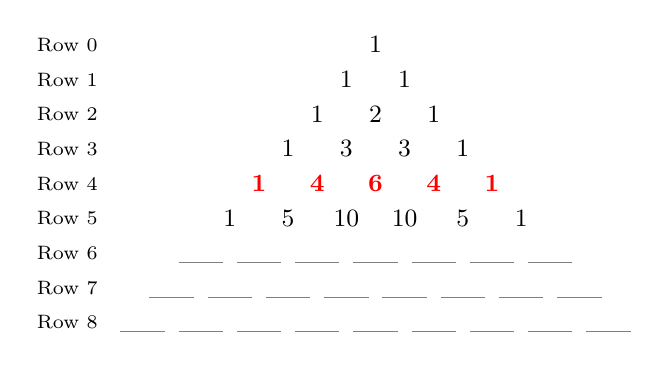
\begin{tikzpicture}[x=0.74cm, y=0.44cm, every node/.style={font=\small}]
\foreach \r/\vals in {0/{1}, 1/{1,1}, 2/{1,2,1}, 3/{1,3,3,1}, 5/{1,5,10,10,5,1}} {
  \node[anchor=east, font=\scriptsize] at (-4.6,-\r) {Row \r};
  \foreach \v [count=\k from 0] in \vals { \node at (\k-\r/2,-\r) {\v}; }
}
\node[anchor=east, font=\scriptsize] at (-4.6,-4) {Row 4};
\foreach \v [count=\k from 0] in {1,4,6,4,1} { \node[red, font=\small\bfseries] at (\k-2,-4) {\v}; }
\foreach \r in {6,7,8} {
  \node[anchor=east, font=\scriptsize] at (-4.6,-\r) {Row \r};
  \pgfmathtruncatemacro{\last}{\r}
  \foreach \k in {0,...,\last} { \draw[gray] (\k-\r/2-0.38,-\r-0.28) -- (\k-\r/2+0.38,-\r-0.28); }
}
\end{tikzpicture}
\end{minipage}\hfill
\begin{minipage}[c]{0.50\textwidth}
\small\setlength{\abovedisplayskip}{3pt}\setlength{\belowdisplayskip}{3pt}
Fill in Rows 6, 7 and 8. If there is no second number above, think of it as 0, so every row starts and ends with 1.

\textbf{Binomial Theorem.} For every positive integer $n$,
\[(a+b)^n=C_0a^n+C_1a^{n-1}b+\cdots+C_nb^n\]
The coefficients $C_0,\dots,C_n$ are the numbers in \textbf{Row $n$}. The powers of $a$ go down, the powers of $b$ go up, and the exponents in each \textbf{term} add to $n$.
\end{minipage}

\vspace{-5pt}
\wspart{Example 5}{Apply the Binomial Theorem}
Use the Binomial Theorem to expand the expressions.
\vspace{-4pt}

\begin{minipage}[t]{0.49\textwidth}
\textbf{A.} Find $(x-3)^4$.
\begin{enumerate}[label=\textbf{\arabic*.}, itemsep=0pt]
\item The exponent is 4, so $n=4$:\\ $C_0a^4+C_1a^3b+C_2a^2b^2+C_3ab^3+C_4b^4$
\item Row 4 (red) gives the coefficients:\\ $a^4+4a^3b+6a^2b^2+4ab^3+b^4$
\item Identify $a$ and $b$: $a=x$ and $b=-3$ (subtracting, so use the opposite of 3).
\item Substitute, then simplify:\\
$x^4+4x^3(-3)+6x^2(-3)^2+4x(-3)^3+(-3)^4$\\
$=x^4+4x^3(-3)+6x^2(9)+4x(-27)+81$\\
$=x^4-12x^3+54x^2-108x+81$
\end{enumerate}
\end{minipage}\hfill
\begin{minipage}[t]{0.48\textwidth}
\textbf{B.} Find $(s^2+3)^5$.
\begin{enumerate}[label=\textbf{\arabic*.}, itemsep=0pt]
\item Row 5: $1,5,10,10,5,1$, so\\ $(a+b)^5=a^5+5a^4b+10a^3b^2+10a^2b^3+5ab^4+b^5$
\item $a=s^2$ and $b=3$.
\item Substitute:\\
$(s^2)^5+5(s^2)^4(3)+10(s^2)^3(3)^2$\\
$\;+10(s^2)^2(3)^3+5(s^2)(3)^4+(3)^5$
\item Simplify (multiply exponents of $s$; $3^2,\dots,3^5$ are $9,27,81,243$):\\
$=s^{10}+15s^8+90s^6+270s^4+405s^2+243$
\end{enumerate}
\end{minipage}

{\small\textbf{Check:} $(a+b)^n$ has $n+1$ terms (5 in A, 6 in B). Signs alternate in A: odd powers of $-3$ are negative.}

\textbf{Say it:} To expand $(x-3)^4$ I used Row \blank[1cm] because the exponent is \blank[1cm]. The coefficients are \blank[3.5cm]. In each term the exponent of $x$ goes \blank[2cm] and the exponents add to \blank[1cm].
\lines[1]

\newpage
\wspart{Try It 5}{Use the Binomial Theorem to expand each expression}
% Try It 5 prompt is the TE sentence verbatim (the heading); the hint is ours.
Hint: Use your Rows 6 and 7. Write the pattern with $a$ and $b$ first, then substitute.

\textbf{a.} $(x-1)^7$

Row 7: \blank[7cm] \qquad $a=\blank[1.5cm]$ \quad $b=\blank[1.5cm]$
\lines[5]

\vspace{6pt}
\textbf{b.} $(2c+d)^6$

Row 6: \blank[7cm] \qquad $a=\blank[1.5cm]$ \quad $b=\blank[1.5cm]$
\lines[6]

\vspace{4pt}
\textbf{Say it:} In part b, why is the first term not $2c^6$? Use the words \emph{coefficient} and \emph{exponent}.
\lines[2]

\newpage
\wspart{IXL}{Practice for the quiz}
Go to IXL, Algebra 2. Type the code in the search box. Do the starred skills first.

\vspace{2pt}
\begin{tabularx}{\textwidth}{l Y Y}
\toprule
\textbf{Code} & \textbf{Skill} & \textbf{Feeds} \\
\midrule
\ixlrow{A7M $\bigstar$}{Pascal's triangle and the Binomial Theorem}{Quiz 4 and 5: pick the row, write the coefficients}
\ixlrow{NEU $\bigstar$}{Binomial Theorem II}{Quiz 4 and 5: substitute $a$ and $b$ (a number, maybe negative), simplify each term}
\ixlrow{G7Y}{Pascal's triangle}{Optional warm-up: build Rows 6--8 (A7M covers the rows the quiz needs)}
\ixlrow{NJV}{Factor sums and differences of cubes}{Optional: Quiz 3 (full Savvas quiz only), Topic 3 test}
\ixlrow{8GN}{Multiply polynomials}{Warm-up from 3-2 for Bonus Quiz 2}
\bottomrule
\end{tabularx}

\vspace{4pt}
\textbf{SmartScore 70 or above on each starred ($\bigstar$) skill replaces your quiz score.}

\vspace{6pt}
\fbox{\parbox{\dimexpr\textwidth-2\fboxsep-2\fboxrule}{\small
\textbf{Reference: the polynomial identities} (Concept Summary)\\[2pt]
\begin{tabular}{@{}ll@{}}
Difference of Squares: $a^2-b^2=(a+b)(a-b)$ & Square of a Sum: $(a+b)^2=a^2+2ab+b^2$ \\
Difference of Cubes: $a^3-b^3=(a-b)(a^2+ab+b^2)$ & Sum of Cubes: $a^3+b^3=(a+b)(a^2-ab+b^2)$
\end{tabular}}}

\wspart{Exit question}{Expand $(x+i)^4$ and justify your work}
% TE Practice & Problem Solving 22 (Example 5, DOK 3, Higher Order Thinking).
Use Pascal's Triangle and the Binomial Theorem to expand $(x+i)^4$. Justify your work.

Row 4: \blank[3.2cm] \quad $a=\blank[1.2cm]$ \quad $b=\blank[1.2cm]$ \quad $i^2=\blank[0.9cm]$ \ $i^3=\blank[0.9cm]$ \ $i^4=\blank[0.9cm]$
\lines[4]

\textbf{Before the quiz, finish these sentences.}

To expand $(a+b)^8$ I use Row \blank[1cm] of Pascal's Triangle, and the expansion has \blank[1cm] terms.

Each \blank[2.5cm] in the expansion comes from the row; the \blank[2.5cm] of $a$ goes down by 1 in each \blank[2cm].

When the binomial is $(x-3)$, I use $b=\blank[1.5cm]$, so the signs of the terms \blank[3cm].

\end{document}
